% isop_rail_auxiliary_supply.tex
% Input-series output-parallel phase-shift full bridges for a 3 kV rail auxiliary supply (model ps_isop_rail of
% modelization-and-control): averaged model, input-voltage sharing with a common phase shift and why transformer
% pairs on one rectifier weaken it, start, flux balance and voltage loop.
% pwr-control template (AAA_template_latex_settings); numbers and figures: isop_rail_auxiliary_supply_analysis.py
% (python3, numpy, scipy, matplotlib, numba; uses isop_sim.py). Compile: pdflatex (three times, for references).
% Rev. 00 - November 2026 - first issue
% Rev. 01 - November 2026 - Sect. 5: controls that keep the input voltages balanced (pair loops on the relative phase), control diagram
\documentclass[10pt,a4paper]{scrartcl}
% ===================== PACKAGES =====================
\usepackage[british]{babel}
\usepackage[tmargin=1in, bmargin=1in, lmargin=0.75in, rmargin=0.75in]{geometry}
\usepackage[dvipsnames,table]{xcolor}  % prima di tikz, listings, ecc.

\usepackage{tikz}
\usepackage{graphicx}
\usepackage{pgfplots}
\pgfplotsset{width=12cm, compat=1.9}
\usepackage{setspace}
\usepackage{chemmacros}
\usepackage{chemfig}
\usepackage{esint}
\usepackage{tabularray}
\usepackage{makeidx}
\usepackage{epstopdf}
\usepackage{amssymb}
\usepackage{mathrsfs}
\usepackage{bm}
\usepackage{amsmath}
\usepackage{enumitem}
\usepackage[english]{varioref}
\usepackage{lipsum}
\usepackage{fancyhdr}
\usepackage{float}
\usepackage{empheq}
\usepackage[framemethod=tikz]{mdframed}
\numberwithin{equation}{section}
\usepackage{eso-pic}
\usepackage{calc}
\usepackage{nccmath}
\usepackage{caption}
\usepackage{subcaption}
\usepackage{gensymb}
\usepackage{amsfonts, amsthm, epsfig, epstopdf, titling, url, array}
\usepackage{tabularx}
\usepackage{makecell}
\usepackage{booktabs}
\usepackage{array}
\usepackage{siunitx}
\sisetup{input-digits=0123456789\pi}
\usepackage[symbol]{footmisc}
\usepackage{multicol}
\usepackage{boondox-cal}
\usepackage{blindtext}
\usepackage{changepage}
\usepackage{nomencl}
\usepackage{hyperref}
\usepackage{xurl}
\usepackage{ragged2e}
\usepackage[version=4]{mhchem}  % ← conflitto di opzioni
\usepackage{longtable}
\usepackage{chemformula}
\usetikzlibrary{arrows.meta,positioning,calc}

% ===================== SI UNITS =====================
\DeclareSIUnit\atm{atm}
\DeclareSIUnit{\var}{var}
\DeclareSIUnit{\pu}{p.u.}


% ===================== MATH OPERATORS =====================
\DeclareMathOperator{\rank}{rank}
\DeclareMathOperator{\atantwo}{atan2}
\DeclareMathOperator{\spn}{span}

% ===================== COMMANDS =====================
\newcommand{\abs}[1]{\left|#1\right|}
\newcommand{\sign}{\text{sign}}
\newcommand{\centered}[1]{\begin{tabular}{@{}l@{}} #1 \end{tabular}}

% ===================== COLORS =====================
\definecolor{mycolor1}{rgb}{0.97, 0.97, 0.97}
\definecolor{mycolor2}{rgb}{0.97, 0.97, 0.97}
\definecolor{tableShade}{gray}{0.9}

% ===================== THEOREM ENVIRONMENTS =====================
\theoremstyle{it}
\newtheorem{defn}{Definition}[section]
\newtheorem{assumption}{Assumption}[section]
\newtheorem{thm}{Theorem}[section]
\newtheorem{lemma}{Lemma}[section]
\newtheorem{corollary}{Corollary}[section]
\theoremstyle{definition}
\newtheorem{example}{Example}[section]

% ===================== CUSTOM ENVIRONMENTS =====================
\newenvironment{myitemize_1}{
	\begin{itemize}[topsep=0pt]
		\setlength{\topsep}{2pt}
		\setlength{\itemsep}{2pt}
		\setlength{\parskip}{2pt}
		\setlength{\parsep}{2pt}
	}{\end{itemize}}

\newmdenv[
innerlinewidth=0.5pt,
roundcorner=4pt,
backgroundcolor=mycolor2,
linecolor=mycolor1,
innerleftmargin=6pt,
innerrightmargin=6pt,
innertopmargin=6pt,
innerbottommargin=6pt
]{mybox}

% ===================== TABLE COLUMN TYPES =====================
\newcolumntype{Y}{>{\hsize=2\hsize}X}
\newcolumntype{Z}{>{\centering\arraybackslash\hsize=0.857\hsize}X}

% ===================== SECTION DEPTH =====================
\setcounter{secnumdepth}{3}
\setcounter{tocdepth}{3}

% ===================== PAGE STYLE =====================
\setlength{\headheight}{20pt}
\setlength{\headsep}{20pt}

\pagestyle{fancy}
\fancypagestyle{firstpage}{\rhead{}}
\fancyhead[L]{\slshape\nouppercase{\leftmark}}
\chead{}
\rhead{\includegraphics[height=0.75cm]{../../AAA_template_latex_settings/pwr-control_logo_doc.png}}
\lfoot{\href{http://www.pwr-control.com}{pwr-control.com}}
\cfoot{-\ \thepage\ -}
\rfoot{\textit{}}
\renewcommand{\headrulewidth}{0.4pt}
\renewcommand{\footrulewidth}{0.4pt}


\geometry{
	a4paper,
	top    = 2.5cm,
	bottom = 3.0cm,
	left   = 2.5cm,
	right  = 2.5cm
}

\hypersetup{
	colorlinks = true,
	urlcolor   = blue,
	linkcolor  = black,
	citecolor  = black
}

\pagenumbering{gobble}
% the document sits three levels below the repository root: logo path of settings.tex corrected here
\rhead{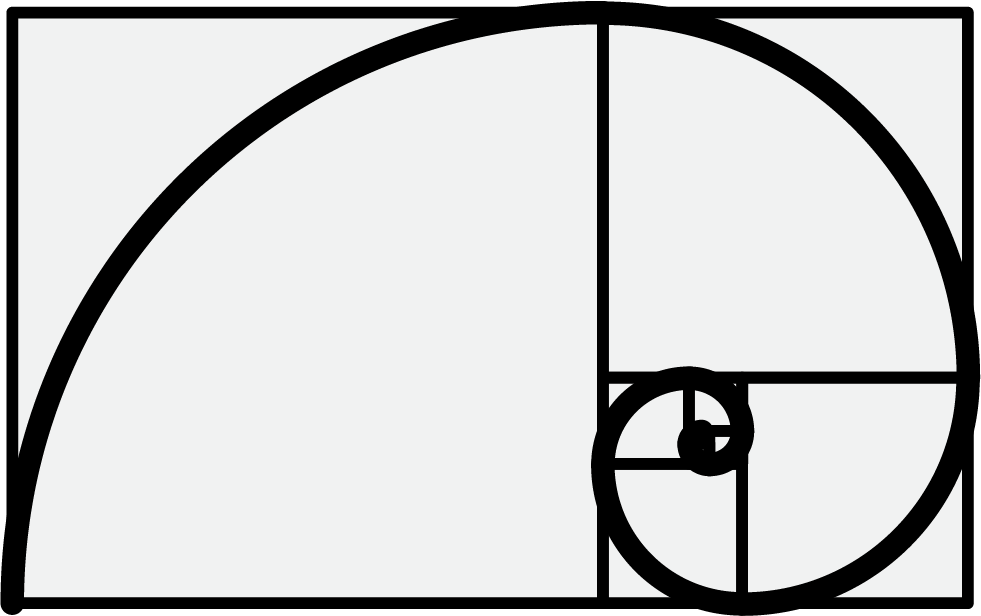
\includegraphics[height=0.75cm]{../../../AAA_template_latex_settings/pwr-control_logo_doc.png}}
\rfoot{\small Rev.~01}
\geometry{left=2.0cm, right=2.0cm}
\usetikzlibrary{arrows.meta,positioning,calc}

\sisetup{per-mode=symbol,range-phrase={\text{--}},range-units=single,retain-explicit-plus}
\setlist{nosep}
\setlength{\parindent}{0pt}
\setlength{\parskip}{3pt}
\allowdisplaybreaks

% --- shorthand ---
\newcommand{\jj}{\mathrm{j}}
\newcommand{\ee}{\mathrm{e}}
\newcommand{\code}[1]{\texttt{#1}}
\newcommand{\Req}{R_{eq}}
\newcommand{\Ls}{L_s}
\newcommand{\vo}{v_o}

% =============================================================
%  DOCUMENT DATA (title page: AAA_template_latex_settings/titlepage.tex)
% =============================================================
\newcommand{\DocCategory}{Technical Note}
\newcommand{\DocField}{Power Electronics and Control Systems}
\newcommand{\DocTitle}{%
	{\fontsize{20}{24}\selectfont\bfseries Input-Series Output-Parallel} \\[12pt]
	{\fontsize{16}{26}\selectfont\bfseries Phase-Shift Full Bridges \\[4pt] for a \SI{3}{kV} Rail Auxiliary Supply \\[8pt] (model \texttt{ps\_isop\_rail})}
}
\newcommand{\DocSubtitle}{Averaged model, input-voltage sharing with a common phase shift, \\[6pt] why transformer pairs on one rectifier weaken it, \\[6pt] balancing controls, start and flux balance}
\newcommand{\DocAuthor}{Davide Bagnara}
\newcommand{\DocRevision}{01}
\newcommand{\DocDate}{November 2026}
\newcommand{\DocAbstract}{%
The model \texttt{ps\_isop\_rail} is a \SI{1}{MW} class auxiliary supply for a \SI{3}{kV} DC catenary: four \SI{250}{kW} phase-shift full bridges in series at the input and in parallel at the output (ISOP), with one output-voltage loop that gives the same phase shift to the four bridges and no input-voltage sharing loop. Its special feature is that the transformers work in pairs: the secondaries of two modules are paralleled on the AC side and feed one diode rectifier. This note derives the averaged model of a module, shows why a common phase shift balances the input voltages of modules on separate rectifiers (time constant \SI{1.2}{ms}) and why the balance almost disappears between two modules on one rectifier: they are tied through leakage reactances, so a voltage difference drives a reactive circulating current and no restoring power. A switched simulation confirms it: \SI{64}{ms} instead of \SI{2.7}{ms}, and a \SI{5}{\percent} leakage difference puts \SI{1351}{V} and \SI{1005}{V} on the two modules of a pair. Rev.~01 adds the controls that restore the balance: a loop per pair on the relative phase of its two bridges and a slow trim of the phase shift between the pairs bring the four voltages within \SI{0.1}{\percent} in about \SI{10}{ms} with \SI{20}{\percent} more leakage in one module, while the classic per-module loop diverges with the modulator of the model. The note also covers the turns ratio, the start, the DC magnetizing current and the voltage loop. A companion Python script reproduces every number and figure.
}
\newcommand{\RevisionHistory}{%
	00 & November 2026 & First issue. & \DocAuthor \\
	01 & November 2026 & Sect.~\ref{sec:control}: balancing controls (control diagram in Fig.~\ref{fig:control}, pair loops on the relative phase, pair-to-pair trim, why the classic per-module loop fails here); power in \eqref{eq:fha} with the factor $1/2$ of peak phasors. & \DocAuthor \\
}
\newcommand{\MetaLabelA}{Project Repository}
\newcommand{\MetaValueAUrl}{https://github.com/pwr-control/modelization-and-control.git}
\newcommand{\MetaValueALabel}{modelization-and-control.git (foundations\_of\_power\_electronics/ps\_isop\_rail)}
\newcommand{\MetaLabelB}{Framework}
\newcommand{\MetaValueB}{MATLAB/Simulink/Simscape; Python 3 (companion script)}

\begin{document}
% =============================================================
%  pwr-control LaTeX template - FRONTESPIZIO
%
%  Da richiamare come prima istruzione dopo \begin{document}:
%      \input{../../AAA_template_latex_settings/titlepage}
%
%  Il documento deve definire prima di \begin{document}:
%      \DocCategory   categoria del documento
%      \DocField      area tecnica
%      \DocTitle      titolo (una o due righe)
%      \DocSubtitle   sottotitolo
%      \DocAuthor     autore/i, separati da virgola
%      \DocRevision   numero di revisione corrente (es. 00)
%      \DocDate       data della revisione corrente
%      \DocAbstract   abstract
%      \RevisionHistory  righe della tabella di revisione, nel formato
%                        Rev. & Date & Description & Authors \\
%      \MetaLabelA \MetaValueAUrl \MetaValueALabel
%      \MetaLabelB \MetaValueB
% =============================================================

\providecommand{\DocCategory}{Technical Research Report}
\providecommand{\DocField}{Power Electronics and Control Systems}
\providecommand{\DocSubtitle}{}
\providecommand{\DocRevision}{00}
\providecommand{\DocAbstract}{}
\providecommand{\RevisionHistory}{%
	\DocRevision & \DocDate & First issue. & \DocAuthor \\
}

\titlepage

% ---- Intestazione centrata ----
\begin{center}
	{\Large\scshape \DocCategory}\\[8pt]
	{\large\scshape \DocField}
\end{center}

\vspace{30pt plus 4pt minus 14pt}
\noindent\rule{\linewidth}{0.8pt}

% ---- Titolo ----
\begin{center}
	\DocTitle
\end{center}

\vspace{4pt}
\noindent\rule{\linewidth}{2.2pt}

% ---- Sottotitolo ----
\begin{center}
	\begin{onehalfspace}
		{\large\itshape \DocSubtitle}
	\end{onehalfspace}
\end{center}

% ---- Authors / Revision / Date ----
\vspace{30pt plus 4pt minus 14pt}

\noindent
\begin{minipage}[t]{0.46\linewidth}
	\raggedright
	\textbf{Authors:}\\[2pt]
	\DocAuthor
\end{minipage}%
\hfill
\begin{minipage}[t]{0.22\linewidth}
	\centering
	\textbf{Revision:}\\[2pt]
	\DocRevision
\end{minipage}%
\hfill
\begin{minipage}[t]{0.30\linewidth}
	\raggedleft
	\textbf{Date:}\\[2pt]
	\DocDate
\end{minipage}

\vspace{10pt}
\noindent\rule{\linewidth}{0.8pt}

% ---- Abstract ----
\vspace{24pt plus 4pt minus 12pt}

\begin{center}
	\begin{minipage}{0.88\linewidth}
		\footnotesize
		\begin{onehalfspace}
			\textbf{Abstract:} \DocAbstract
		\end{onehalfspace}
	\end{minipage}
\end{center}

\vfill

% ---- Revision history ----
\begin{center}
	\begin{minipage}{0.96\linewidth}
		\centering
		{\footnotesize\scshape Revision history}\\[6pt]
		{\footnotesize
			\begin{tabular}{@{}cl>{\raggedright\arraybackslash}p{0.36\linewidth}>{\raggedright\arraybackslash}p{0.28\linewidth}@{}}
				\toprule
				\textbf{Rev.} & \textbf{Date} & \textbf{Description} & \textbf{Authors} \\
				\midrule
				\RevisionHistory
				\bottomrule
			\end{tabular}}
	\end{minipage}
\end{center}

\vspace{18pt plus 4pt minus 10pt}

% ---- Metadati in fondo ----
\noindent
\begin{tabular}{@{} r @{\quad} l @{}}
	\textsc{\MetaLabelA:} & {\href{\MetaValueAUrl}{\MetaValueALabel}} \\[3pt]
	\textsc{\MetaLabelB:} & {\MetaValueB}       \\[3pt]
\end{tabular}

% =============================================================
%  Fine frontespizio
% =============================================================
\newpage
\pagenumbering{arabic}
\setcounter{page}{1}

\tableofcontents
\newpage
\begin{onehalfspace}

% =====================================================================================================
\section{Scope}
\label{sec:scope}

The model \code{ps\_isop\_rail} (\path{foundations_of_power_electronics/ps_isop_rail} of modelization-and-control) is an auxiliary power supply for a \SI{3}{kV} DC railway catenary. The catenary voltage (\SIrange{2000}{3600}{V} of permanent range in EN~50163 \cite{en50163}) is too high for one bridge with \SI{1.7}{kV} devices, so four isolated modules share it in series at the input and give a common \SI{750}{V} output in parallel (input series, output parallel: ISOP). Each module is a phase-shift full bridge (PSFB) \cite{sabate1990}; one voltage loop gives the same phase shift to the four bridges (common-duty control \cite{giri2006}) and there is no input-voltage sharing loop.

During the migration of the model to the parameter structure of the repository (November 2026, pull request \#26 of modelization-and-control) a design check with a switched simulation of the whole circuit was made. This note collects it: Sect.~\ref{sec:system} gives the system, Sect.~\ref{sec:averaged} the averaged model of a module and the turns ratio, Sect.~\ref{sec:sharing} the input-voltage sharing (the main point), Sect.~\ref{sec:control} the controls that keep it balanced (added in rev.~01), Sect.~\ref{sec:start} the start, the flux balance and the voltage loop, Sect.~\ref{sec:summary} the summary. Every number comes from the companion script \code{isop\_rail\_auxiliary\_supply\_analysis.py}, which uses the switched simulator \code{isop\_sim.py} (the same circuit and values as \code{init\_model.m} of the model: backward Euler at \SI{0.625}{\micro s} like the Simscape local solver, ideal switches and piecewise-linear diodes, the modulator and the voltage PI of the model).

% =====================================================================================================
\section{The system}
\label{sec:system}

Fig.~\ref{fig:system} shows the power stage and Table~\ref{tab:data} the data. A lithium-ion battery emulates the catenary; it is set to $1.5$ times the catenary voltage (\SI{4696}{V} open circuit), a choice that Sect.~\ref{sec:ratio} explains. The four input capacitors are in series; each one feeds its own full bridge and transformer. The secondaries of modules 1 and 4 are paralleled on the AC side and feed rectifier~1, those of modules 2 and 3 feed rectifier~2; each rectifier has its own \SI{250}{\micro H} inductor and the two share the output capacitor and the load.

\begin{figure}[htb]
\centering
\begin{tikzpicture}[x=1cm,y=1cm,font=\small,>=Stealth,
	blk/.style={draw,rounded corners=2pt,align=center,fill=white,inner sep=3pt},
	ac/.style={line width=1.4pt}]
\foreach \k/\y in {1/2.55,2/0.85,3/-0.85,4/-2.55} {
	\node[blk,minimum width=3.7cm,minimum height=1.15cm] (m\k) at (4.3,\y) {module \k\\[-1pt]{\footnotesize $C_{in}$, full bridge, $T_{\k}$ (1:1)}};
	\draw (m\k.west) ++(0,0.34) -- ++(-0.45,0) coordinate (p\k);
	\draw (m\k.west) ++(0,-0.34) -- ++(-0.45,0) coordinate (n\k);
}
\draw (n1) -- (p2) (n2) -- (p3) (n3) -- (p4);
\node[blk,minimum width=1.9cm,minimum height=2.4cm] (bat) at (-0.6,0) {catenary\\emulator\\\SI{4.5}{kV}\\(battery)};
\coordinate (bp) at ($(bat.east)+(0,0.8)$);
\coordinate (bn) at ($(bat.east)+(0,-0.8)$);
\draw (p1) -- ++(-0.5,0) coordinate (a1) |- (bp);
\node[left,font=\footnotesize,align=right] at ($(a1)+(-0.05,-0.85)$) {\SI{1}{mH} line\\+ \SI{1}{mH} $L_{in}$};
\draw (n4) -- ++(-0.5,0) |- (bn);
\node[blk,minimum width=1.9cm,minimum height=1.0cm] (r1) at (9.4,1.7) {rectifier 1};
\node[blk,minimum width=1.9cm,minimum height=1.0cm] (r2) at (9.4,-1.7) {rectifier 2};
\draw[ac] (m1.east) -- (7.3,2.55) |- ($(r1.west)+(0,0.22)$);
\draw[ac] (m4.east) -- (7.9,-2.55) |- ($(r1.west)+(0,-0.22)$);
\draw[ac] (m2.east) -- (7.0,0.85) |- ($(r2.west)+(0,0.22)$);
\draw[ac] (m3.east) -- (6.7,-0.85) |- ($(r2.west)+(0,-0.22)$);
\node[font=\footnotesize,align=center] at (7.6,3.1) {AC side};
\node[blk,minimum width=2.2cm,minimum height=1.6cm] (out) at (13.6,0) {$C_{out}$ \SI{1.2}{mF}\\load \SI{0.5}{\ohm}\\\SI{750}{V}};
\draw (r1.east) -- node[above,font=\footnotesize]{\SI{250}{\micro H}} (11.8,1.7) |- ($(out.west)+(0,0.3)$);
\draw (r2.east) -- node[below,font=\footnotesize]{\SI{250}{\micro H}} (11.8,-1.7) |- ($(out.west)+(0,-0.3)$);
\end{tikzpicture}
\caption{Power stage of \code{ps\_isop\_rail}: four modules in series at the input; the transformers of modules 1+4 and 2+3 are paralleled on the AC side (thick lines), one diode rectifier and one inductor per pair, common output capacitor.}
\label{fig:system}
\end{figure}

\begin{table}[htb]
\centering
\caption{Data of the model (values of \code{init\_model.m}).}
\label{tab:data}
\small
\begin{tabularx}{\textwidth}{@{}l>{\raggedright\arraybackslash}X@{}}
\toprule
Item & Value \\
\midrule
catenary emulator & battery, \SI{4500}{V} nominal, \SI{4696}{V} open circuit (soc 0.85), \SI{1}{mH} line; string inductor $L_{in}$ \SI{1}{mH} \\
module & \SI{250}{kW}; $C_{in}$ \SI{1.2}{mF}; full bridge of ideal switches (\SI{1.5}{m\ohm}), \SI{4}{kHz}, dead time \SI{3}{\micro s} \\
transformer & $n = 1$, $L_m = \SI{1}{mH}$, leakage $\Ls = \SI{26.0}{\micro H}$ referred to the primary (half on each side), \SI{1}{m\ohm} per winding \\
output & two diode rectifiers, \SI{250}{\micro H} each, $C_{out}$ \SI{1.2}{mF}, load \SI{0.5}{\ohm}: \SI{750}{V}, \SI{1500}{A}, \SI{1.125}{MW} (\SI{112}{\percent} of $4\times\SI{250}{kW}$) \\
control & \SI{8}{kHz} (two updates per carrier period); voltage PI $k_p = 0.5$, $k_i = \SI{18}{s^{-1}}$, output = phase shift $D \in [0,1]$ (pu of $\pi$) of the four bridges; reference \SI{750}{V} applied as a step \\
\bottomrule
\end{tabularx}
\end{table}

% =====================================================================================================
\section{Averaged model of a module}
\label{sec:averaged}

\subsection{Duty-cycle loss and output resistance}

With the phase shift $D$ the bridge puts $\pm v_k$ on the primary for the fraction $D$ of each half period. The secondary current is the inductor current $i_k$ (ripple neglected); at each change of polarity the primary current must go from $+n\,i_k$ to $-n\,i_k$ through the leakage, under the full voltage $v_k$, and during that time the rectifier short-circuits the secondary. The lost fraction of the half period is
\begin{equation}
\Delta D = \frac{2\,n\,i_k\,\Ls}{v_k}\cdot 2f = \frac{4\,n\,\Ls\,f\,i_k}{v_k},
\end{equation}
so the rectified output and the input current of module $k$ are
\begin{equation}
\vo = n\,v_k\,(D - \Delta D) = n\,D\,v_k - \Req\,i_k, \qquad \Req = 4\,n^2\,\Ls\,f, \qquad i_{in,k} = n\,(D-\Delta D)\,i_k = \frac{\vo\,i_k}{v_k}.
\label{eq:avg}
\end{equation}
$\Req$ is a lossless resistance that models the duty-cycle loss \cite{sabate1990}: here $\Req = \SI{0.417}{\ohm}$, which costs \SI{156}{V} at the \SI{375}{A} of one module. At the operating point (\SI{1171}{V} per module) the phase shift is $D = 0.777$ (the switched simulation gives 0.782). Fig.~\ref{fig:waveforms} shows the switched waveforms there: the primary current reverses through the leakage at each change of polarity of the bridge voltage (the duty-cycle loss), the magnetizing current is small (\SI{52}{A} peak against \SI{460}{A}), and the two secondaries of a pair carry the same current when the modules are equal. Each module has \SI{1170.9}{V} and \SI{380}{A} rms in its primary, and each rectifier gives \SI{751.5}{A}.

\begin{figure}[htb]
\centering
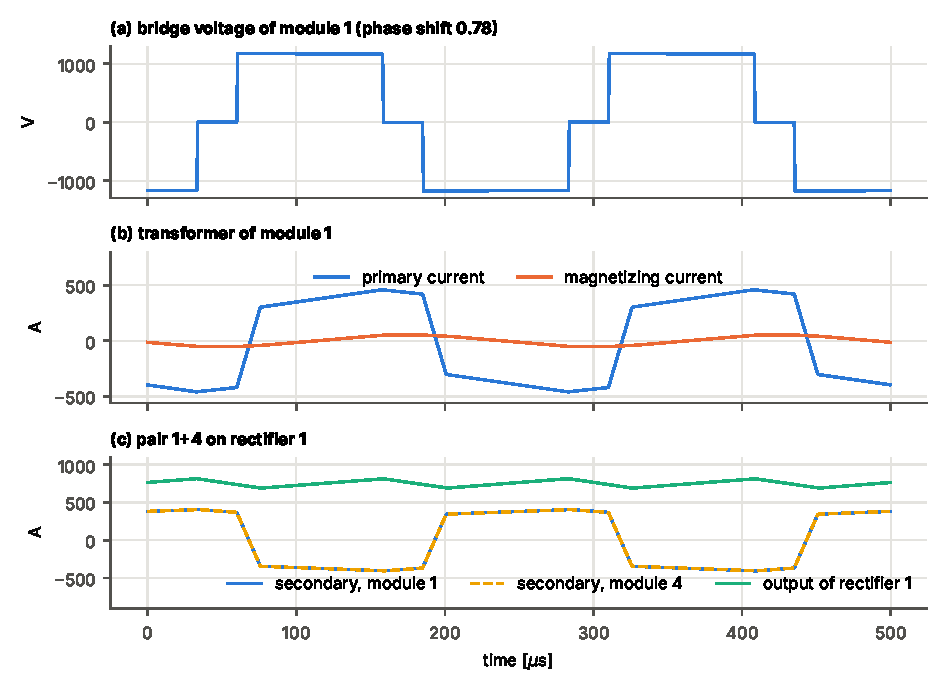
\includegraphics[width=0.74\textwidth]{figures/fig_waveforms.pdf}
\caption{Steady state with identical modules (switched simulation): bridge voltage, primary and magnetizing current of module 1, secondary currents of the pair 1+4 and output current of rectifier 1.}
\label{fig:waveforms}
\end{figure}

\subsection{Turns ratio, leakage and catenary voltage}
\label{sec:ratio}

With $n = 1$ and this leakage a module needs about \SI{1170}{V} to give \SI{750}{V}: that is why the emulator is set to $1.5$ times the catenary. At the nominal \SI{3}{kV} (\SI{750}{V} per module) the largest output at full load is \SI{591}{V}; the simulation with the emulator at \SI{3}{kV} stops at \SI{604}{V} with the PI saturated (Fig.~\ref{fig:start}a). The leakage was sized with the formula of a dual active bridge (maximum power $V_1V_2/(8f\Ls) = 2.7\,P$), but in a PSFB the leakage does not transfer power: it gives the soft switching and the duty-cycle loss. A PSFB is sized the other way round: the turns ratio from the lowest catenary voltage at which full output is needed, the leakage from an allowed duty-cycle loss. With a largest phase shift of 0.9 and \SI{10}{\percent} duty-cycle loss: $n = 1.24$ and $\Ls = \SI{9.1}{\micro H}$ for full output at \SI{3}{kV}, $n = 1.85$ and $\Ls = \SI{4.05}{\micro H}$ at \SI{2}{kV}. The soft switching of the lagging leg at light load then sets a lower limit to $\Ls$ \cite{sabate1990}.

% =====================================================================================================
\section{Input-voltage sharing with a common phase shift}
\label{sec:sharing}

The modules are in series at the input, so they carry the same string current. In steady state each input capacitor has zero average current, so each module must draw the same average input current; the input voltages settle where this is true. Whether they settle at equal values, and how fast, depends on how a module's input current reacts to its own input voltage.

\subsection{Modules on separate rectifiers: a resistive coupling}

With separate rectifiers the modules meet on the DC side. With $D$ common and $\vo$ held by the output capacitor, \eqref{eq:avg} gives $i_k = (n D v_k - \vo)/\Req$ and
\begin{equation}
\frac{\partial i_{in,k}}{\partial v_k} = g = \frac{\vo}{v_k}\left(\frac{n\,D}{\Req} - \frac{i_k}{v_k}\right) = 0.6405\,(1.864 - 0.320)\,\si{S} = \SI{0.989}{S}.
\end{equation}
A module whose voltage rises gives more output current, draws more input current and discharges its capacitor: every difference between the module voltages decays with $\tau = C_{in}/g = \SI{1.2}{ms}$ (first order; the output inductors make the decay oscillating). This is the known self-balancing of ISOP modules with a common duty ratio \cite{giri2006}. The coupling goes through $\Req$, which acts like a resistance: it moves real power from the module with the higher voltage. A mismatch only shifts the balance a little: in the averaged steady state a module with \SI{20}{\percent} more leakage settles at \SI{1208}{V} against \SI{1158}{V} for the others (\SI{+3}{\percent}).

\subsection{Two modules on one rectifier: a reactive coupling}

In a pair the two transformers meet on the AC side, before the rectifier. With the fundamental-harmonic model each bridge is a voltage source in phase with the other (same carrier and phase shift), of peak value $V_k = \tfrac{4}{\pi}\,v_k \sin(\pi D/2)$, connected through its leakage reactance $X_k = 2\pi f\,\Ls n^2$ (referred to the secondary) to the rectifier input, of voltage $V_r\,\ee^{-\jj\theta}$ (peak phasors). The current and the real power of module $k$ are
\begin{equation}
\underline{I}_k = \frac{n V_k - V_r\,\ee^{-\jj\theta}}{\jj X_k}, \qquad P_k = \tfrac{1}{2}\mathrm{Re}\{n V_k\,\underline{I}_k^*\} = \frac{n\,V_k\,V_r\sin\theta}{2X_k}, \qquad i_{in,k} = \frac{P_k}{v_k} = \frac{2\,n\sin(\pi D/2)\,V_r\sin\theta}{\pi\,X_k}.
\label{eq:fha}
\end{equation}
The input current does not depend on $v_k$: there is no restoring term. A difference $n(V_a - V_b)$ between the two bridges of a pair drives a circulating current $n(V_a - V_b)/(\jj(X_a + X_b))$ in quadrature with the bridge voltages: reactive power, no real power. Only second-order effects (winding and switch resistances, the commutation of the rectifier) give some restoring power. And \eqref{eq:fha} shows that the leakage enters directly: the module with the larger $X_k$ draws less input current, its capacitor charges and its voltage rises until the weak second-order terms balance the difference. A turns-ratio difference is harmless: the circulating current vanishes when $n_a v_a = n_b v_b$, and the pair settles there.

The four-winding transformer derived in \path{ps_isop_rail/trafo} (two primaries and two secondaries on one core) puts the two bridges of a pair on the same flux, so they are again tied through leakage reactances; it can save a core but it should have the same weak sharing (not simulated).

\subsection{Switched simulation}

Fig.~\ref{fig:sharing} and Table~\ref{tab:sharing} give the sharing; with identical modules it is perfect. With the phase shift fixed at the operating point and \SI{80}{V} of initial deviation, the deviation between the two pairs decays with an envelope time constant of \SI{2.7}{ms} (oscillating, through the output inductors), the deviation inside a pair with \SI{64}{ms}, about 23 times slower. A \SI{5}{\percent} leakage difference inside a pair puts \SI{1351}{V} and \SI{1005}{V} on its two modules (\SI{+15}{\percent} and \SI{-14}{\percent}); \SI{20}{\percent} gives \SI{1450}{V} and \SI{959}{V}, and the module with the higher voltage carries about \SI{357}{kW} (\SI{143}{\percent} of its rating) with \SI{606}{A} rms and \SI{900}{A} peak in its primary. The turns-ratio case settles at equal $n\,v$, as expected.

\begin{figure}[htb]
\centering
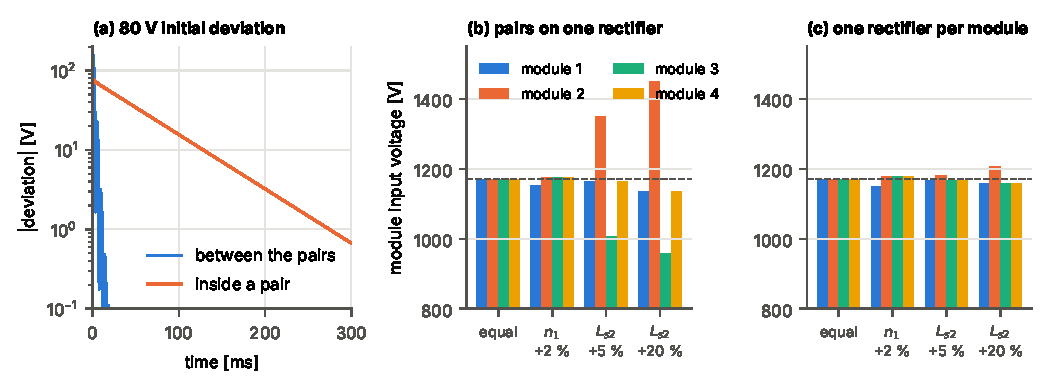
\includegraphics[width=\textwidth]{figures/fig_sharing.pdf}
\caption{Input-voltage sharing. (a) Decay of an \SI{80}{V} deviation at the operating point (phase shift fixed): between the pairs and inside a pair. (b) Steady-state module voltages of the model with one module different (switched simulation). (c) The same with one rectifier per module (averaged model \eqref{eq:avg}).}
\label{fig:sharing}
\end{figure}

\begin{table}[htb]
\centering
\caption{Steady-state input voltages of the modules with one module different.}
\label{tab:sharing}
\small
\begin{tabular}{@{}lll@{}}
\toprule
Case & Pairs on one rectifier (switched simulation) & One rectifier per module (averaged) \\
\midrule
equal modules & \SI{1171}{V} on each module & \SI{1171}{V} on each module \\
module 1: $n$ \SI{+2}{\percent} & module 1 \SI{1153}{V}, the others \SI{1177}{V} & \SI{1150}{V} / \SI{1178}{V} \\
module 2: $\Ls$ \SI{+5}{\percent} & module 2 \SI{1351}{V}, module 3 \SI{1005}{V}, 1 and 4 \SI{1164}{V} & \SI{1180}{V} / \SI{1168}{V} \\
module 2: $\Ls$ \SI{+20}{\percent} & module 2 \SI{1450}{V}, module 3 \SI{959}{V}, 1 and 4 \SI{1137}{V} & \SI{1208}{V} / \SI{1158}{V} \\
\bottomrule
\end{tabular}
\end{table}

\subsection{Remedies}

\begin{enumerate}
\item \textbf{One rectifier per module.} Two more rectifiers and inductors, and the modules meet on the DC side again: the classic ISOP with the resistive coupling of the first subsection (\SI{+3}{\percent} for a \SI{20}{\percent} leakage difference).
\item \textbf{Balancing loops} (Sect.~\ref{sec:control}). A duty correction changes mainly the amplitude of a bridge voltage, which in a pair gives reactive current again. A small time shift $\varphi$ between the two bridges of a pair moves real power through the leakages, as in a dual active bridge \cite{dedoncker1991}; a PI on $v_a - v_b$ that sets $\varphi$, plus a slow trim of the phase shift between the pairs, restores the sharing. The modulator then needs one carrier per bridge instead of one for all.
\end{enumerate}

% =====================================================================================================
\section{Controls that keep the input voltages balanced}
\label{sec:control}

Sect.~\ref{sec:sharing} showed that a common phase shift keeps the two pairs balanced against each other, but hardly the two modules inside a pair. This section (added in rev.~01) proposes a control that does it, tests it in the switched simulation and explains why the classic per-module loop of the ISOP literature fails in this circuit. Fig.~\ref{fig:control}a shows the whole control, Fig.~\ref{fig:control}b what its two handles do in the modulator.

\begin{figure}[!htb]
\centering
\begin{tikzpicture}[x=1cm,y=1cm,>=Latex,font=\footnotesize,
	blk/.style={draw,align=center,fill=gray!12,inner sep=2pt,minimum height=0.62cm},
	bal/.style={blk,fill=RoyalBlue!14},
	pwr/.style={draw,align=center,fill=white,inner sep=2pt},
	sum/.style={draw,circle,minimum size=3.4mm,inner sep=0pt,fill=white},
	lbl/.style={inner sep=1pt,font=\scriptsize},
	bus/.style={line width=1.8pt,draw=gray!55},
	ac/.style={line width=1.3pt}]
\node[font=\small,anchor=west] at (-0.2,5.3) {(a)};
% legend
\node[blk,minimum width=0.3cm,minimum height=0.22cm,inner sep=0pt] at (1.2,5.3) {};
\node[lbl,anchor=west] at (1.4,5.3) {in the model};
\node[bal,minimum width=0.3cm,minimum height=0.22cm,inner sep=0pt] at (3.35,5.3) {};
\node[lbl,anchor=west] at (3.55,5.3) {balancing loops of this section (not in the model)};
% ------------------------------------------------------------------ output-voltage loop (the model)
\node[sum] (s0) at (1.75,4.45) {};
\node[lbl,anchor=west] (ref) at (-0.2,4.45) {$v_o^*$ \SI{750}{V}};
\draw[->] (ref) -- (s0);
\draw[->] (0.15,4.0) -- node[lbl,above,pos=0.4]{$v_o$} (1.75,4.0) -- (s0.south);
\node[blk,minimum width=1.3cm] (piv) at (3.2,4.45) {PI$_v$\\[-2pt]{\scriptsize $[0,\,1]$}};
\draw[->] (s0) -- (piv);
% ------------------------------------------------------------------ pair-to-pair loop
\node[sum] (s1) at (1.75,3.25) {};
\draw[->] (0.15,3.25) -- node[lbl,above,pos=0.4]{$\bar v_1{+}\bar v_4$} (s1);
\draw[->] (0.15,2.8) -- node[lbl,above,pos=0.4]{$\bar v_2{+}\bar v_3$} (1.75,2.8) -- (s1.south);
\node[bal,minimum width=1.3cm] (pid) at (3.2,3.25) {PI$_d$\\[-2pt]{\scriptsize $\pm 0.05$}};
\draw[->] (s1) -- (pid);
\node[bal,minimum width=1.05cm,minimum height=1.75cm] (dd) at (5.0,3.85) {$D + d$\\[20pt]$D - d$};
\draw[->] (piv) -- node[lbl,above]{$D$} (piv -| dd.west);
\draw[->] (pid) -- node[lbl,above]{$d$} (pid -| dd.west);
% ------------------------------------------------------------------ pair loops
\foreach \r/\a/\b/\p/\c/\e/\y in {2/1/4/14/2/4/1.85, 3/2/3/23/3/3/0.45} {
	\node[sum] (s\r) at (1.75,\y) {};
	\draw[->] (0.15,\y) -- node[lbl,above,pos=0.4]{$\bar v_{\a}$} (s\r);
	\draw[->] (0.15,\y-0.45) -- node[lbl,above,pos=0.4]{$\bar v_{\b}$} (1.75,\y-0.45) -- (s\r.south);
	\node[bal,minimum width=1.3cm] (pip\r) at (3.2,\y) {PI$_\varphi$\\[-2pt]{\scriptsize $\pm\SI{0.2}{rad}$}};
	\draw[->] (s\r) -- (pip\r);
	\node[bal,minimum width=1.05cm,minimum height=0.95cm] (h\r) at (5.0,\y) {$-\tfrac{1}{2}$\\[3pt]$+\tfrac{1}{2}$};
	\draw[->] (pip\r) -- node[lbl,above]{$\varphi_{\p}$} (h\r);
}
% signs at the summing junctions
\foreach \r in {0,1,2,3} {
	\node[lbl] at ($(s\r.west)+(-0.1,0.14)$) {$+$};
	\node[lbl] at ($(s\r.south)+(0.15,-0.13)$) {$-$};
}
% ------------------------------------------------------------------ modulators
\node[bal,minimum width=2.2cm,minimum height=5.4cm,anchor=south,font=\scriptsize] (mod) at (8.65,-0.55) {%
	{\footnotesize PSFB}\\[-1pt]{\footnotesize modulators}\\[5pt]
	one \SI{4}{kHz} carrier\\[-1pt] per bridge\\[5pt]
	bridge $k$:\\[-1pt] leg A delayed by $\delta_k$,\\[-1pt] leg B by $\delta_k + \pi D_k$\\[5pt]
	$D_1 = D_4 = D_{14}$\\[-1pt] $D_2 = D_3 = D_{23}$\\[5pt]
	dead time \SI{3}{\micro s}};
\draw[->] (dd.east |- 0,4.45) -- node[lbl,above]{$D_{14} = D + d$} (mod.west |- 0,4.45);
\draw[->] (dd.east |- 0,3.25) -- node[lbl,above]{$D_{23} = D - d$} (mod.west |- 0,3.25);
\draw[->] (h2.east |- 0,2.1) -- node[lbl,above]{$\delta_1 = -\varphi_{14}/2$} (mod.west |- 0,2.1);
\draw[->] (h2.east |- 0,1.6) -- node[lbl,above]{$\delta_4 = +\varphi_{14}/2$} (mod.west |- 0,1.6);
\draw[->] (h3.east |- 0,0.7) -- node[lbl,above]{$\delta_2 = -\varphi_{23}/2$} (mod.west |- 0,0.7);
\draw[->] (h3.east |- 0,0.2) -- node[lbl,above]{$\delta_3 = +\varphi_{23}/2$} (mod.west |- 0,0.2);
% ------------------------------------------------------------------ power stage
\draw[dashed,rounded corners=3pt,gray] (10.5,-1.0) rectangle (16.75,5.45);
\node[lbl,anchor=north east,gray!70!black] at (16.7,5.4) {power stage (Fig.~\ref{fig:system})};
\foreach \k/\y in {1/4.25,2/2.85,3/1.45,4/0.05} {
	\node[pwr,minimum width=1.6cm,minimum height=0.8cm] (m\k) at (11.55,\y) {module \k\\[-2pt]{\scriptsize $v_{\k}$, bridge, $T_{\k}$}};
	\draw[->] (mod.east |- m\k) -- (m\k.west);
}
\node[lbl,above] at (10.25,4.25) {gates};
\draw (m1.north) -- ++(0,0.3) node[lbl,above]{catenary};
\draw (m1.south) -- (m2.north) (m2.south) -- (m3.north) (m3.south) -- (m4.north);
\draw (m4.south) -- ++(0,-0.3) node[lbl,below]{rail};
\node[pwr,minimum width=1.1cm,minimum height=0.75cm] (r1) at (13.95,3.55) {rect.~1};
\node[pwr,minimum width=1.1cm,minimum height=0.75cm] (r2) at (13.95,0.75) {rect.~2};
\draw[ac] (m1.east) -- (12.9,4.25) |- ($(r1.west)+(0,0.15)$);
\draw[ac] (m4.east) -- (13.1,0.05) |- ($(r1.west)+(0,-0.15)$);
\draw[ac] (m2.east) -- (12.75,2.85) |- ($(r2.west)+(0,0.15)$);
\draw[ac] (m3.east) -- (12.6,1.45) |- ($(r2.west)+(0,-0.15)$);
\node[pwr,minimum width=1.45cm,minimum height=1.2cm] (out) at (15.8,2.15) {$C_{out}$\\[-1pt]load\\[-1pt]$v_o$};
\draw (r1.east) -- (14.85,3.55) |- ($(out.west)+(0,0.25)$);
\draw (r2.east) -- (14.85,0.75) |- ($(out.west)+(0,-0.25)$);
% ------------------------------------------------------------------ measurements
\node[blk,minimum width=2.6cm] (adc) at (6.6,-1.55) {sampled at \SI{8}{kHz},\\[-2pt] one sample of delay};
\node[bal,minimum width=2.8cm] (avg) at (3.0,-1.55) {mean over a period\\[-2pt] $\bar v_k = \tfrac{1}{2}(1 + z^{-1})\,v_k$};
\draw[bus,-{Latex[length=2.6mm]}] (13.95,-1.0) -- (13.95,-1.55) -- (adc.east);
\draw[bus,-{Latex[length=2.6mm]}] (adc.west) -- (avg.east);
\draw[bus] (avg.west) -- (0.15,-1.55) -- (0.15,4.0);
\node[lbl,above] at (11.4,-1.55) {$v_1 \ldots v_4$, $v_o$};
\node[lbl,above] at (0.85,-1.55) {$\bar v_k$, $v_o$};
\foreach \y in {4.0,3.25,2.8,1.85,1.4,0.45,0.0} {\fill (0.15,\y) circle (1.4pt);}
\end{tikzpicture}

\vspace{8pt}
\begin{tikzpicture}[x=1cm,y=1cm,>=Latex,font=\scriptsize]
\node[font=\small,anchor=west] at (-3.2,3.45) {(b)};
% time scale: T = 8 cm; sketch with D = 0.6 (D T/2 = 2.4 cm) and a relative shift of 0.4 cm (phi exaggerated)
\draw[thick] (0,2.7) -- (0.8,2.7) -- (0.8,3.1) -- (4.8,3.1) -- (4.8,2.7) -- (8.8,2.7) -- (8.8,3.1) -- (9.2,3.1);
\node[anchor=east] at (-0.15,2.9) {leg A, bridge $a$};
\draw[thick] (0,1.85) -- (3.2,1.85) -- (3.2,2.25) -- (7.2,2.25) -- (7.2,1.85) -- (9.2,1.85);
\node[anchor=east] at (-0.15,2.05) {leg B, bridge $a$};
\draw[thick] (0,1.0) -- (0.8,1.0) -- (0.8,1.35) -- (3.2,1.35) -- (3.2,1.0) -- (4.8,1.0) -- (4.8,0.65) -- (7.2,0.65) -- (7.2,1.0) -- (8.8,1.0) -- (8.8,1.35) -- (9.2,1.35);
\node[anchor=east] at (-0.15,1.0) {$v_{AB}$, bridge $a$};
\draw[thick,RoyalBlue] (0,-0.2) -- (1.2,-0.2) -- (1.2,0.15) -- (3.6,0.15) -- (3.6,-0.2) -- (5.2,-0.2) -- (5.2,-0.55) -- (7.6,-0.55) -- (7.6,-0.2) -- (9.2,-0.2);
\node[anchor=east,RoyalBlue] at (-0.15,-0.2) {$v_{AB}$, bridge $b$};
% carrier phase without balancing (delta = 0)
\draw[densely dotted] (1.0,-0.75) -- (1.0,3.25);
\node[anchor=north] at (1.0,-0.75) {$\delta = 0$};
% period and phase shift
\draw[<->] (0.8,3.3) -- node[above]{$T = \SI{250}{\micro s}$} (8.8,3.3);
\draw[densely dotted] (0.8,2.7) -- (0.8,1.85);
\draw[<->] (0.8,2.45) -- node[fill=white,inner sep=1pt]{$D\,T/2$} (3.2,2.45);
% relative shift of the two bridges of the pair
\draw[densely dotted] (0.8,1.0) -- (0.8,-0.2);
\draw[->] (0.3,0.42) -- (0.8,0.42);
\draw[->] (1.7,0.42) -- (1.2,0.42);
\node[anchor=west] at (1.75,0.42) {$\varphi\,T/2\pi$};
\end{tikzpicture}
\caption{Control with the balancing loops. (a) Block diagram: the output-voltage loop of the model gives the common phase shift $D$; the balancing loops of this section add a trim $\pm d$ of the phase shift between the pairs and, inside each pair, opposite carrier delays $\delta_k = \mp\varphi/2$ (rad of the switching period, negative: earlier) from a PI on the voltage difference of its two modules. All loops run at \SI{8}{kHz} with one sample of delay; the module voltages are averaged over one switching period. Thick lines: AC side. (b) Modulation of the two bridges $a$ and $b$ of a pair (sketch with $D = 0.6$, shift exaggerated): the phase shift moves leg B only and sets the width $D\,T/2$ of the voltage pulses (the amplitude); the carrier delays $\delta_a = -\varphi/2$ and $\delta_b = +\varphi/2$ move both legs and shift the pulses by $\varphi\,T/2\pi$ (the angle).}
\label{fig:control}
\end{figure}

\subsection{Two handles per bridge}

Each bridge has two handles: its phase shift $D$, the width of its voltage pulses, which sets the amplitude $V_k$ of \eqref{eq:fha}; and the phase of its carrier (both legs moved together), which sets the angle of its voltage (Fig.~\ref{fig:control}b). Inside a pair the two bridges are two voltage sources on one AC node, each behind its leakage reactance, like two generators on one bus: real power follows the angle, while the amplitude moves mainly reactive power. If the voltages of the two bridges of a pair are moved by $+\varphi/2$ and $-\varphi/2$ in angle (carrier delays $\delta = \mp\varphi/2$), \eqref{eq:fha} gives
\begin{equation}
i_{in,a} - i_{in,b} \approx K_\varphi\,\varphi, \qquad K_\varphi = \frac{2\,n\sin(\pi D/2)\,V_r\cos\theta}{\pi X} = \SI{838}{A/rad},
\label{eq:kphi}
\end{equation}
with $V_r = 4\vo/\pi = \SI{955}{V}$, $X = \SI{0.654}{\ohm}$ and the load angle $\theta = \ang{16}$ (from $P_k$ in \eqref{eq:fha}). The \SI{44}{A} input-current difference that \SI{20}{\percent} more leakage causes in one bridge (at equal module voltages) needs only $\varphi \approx \ang{3}$, a time shift of \SI{2}{\micro s} between the two carriers. A trim of the phase shift of one bridge, with its angle fixed, moves only $K_A = i_{in}\,(\pi/2)\cot(\pi D/2) = \SI{138}{A}$ per unit: the same case would need $\pm 0.16$ on the two bridges.

\subsection{Pair loops and pair-to-pair trim}

The proposed control (Fig.~\ref{fig:control}a) adds three slow loops to the output-voltage loop, which keeps the common phase shift $D$:
\begin{equation}
\varphi_{14} = \mathrm{PI}_\varphi\{\bar v_1 - \bar v_4\}, \qquad \varphi_{23} = \mathrm{PI}_\varphi\{\bar v_2 - \bar v_3\}, \qquad d = \mathrm{PI}_d\{(\bar v_1 + \bar v_4) - (\bar v_2 + \bar v_3)\}.
\end{equation}
The carrier of bridge 1 moves earlier by $\varphi_{14}/2$ and that of bridge 4 later by $\varphi_{14}/2$ (the same for bridges 2 and 3 with $\varphi_{23}$), so the bridge with the higher input voltage leads and takes more power; pair 1+4 gets the phase shift $D + d$ and pair 2+3 gets $D - d$. Here $\bar v_k$ is the input voltage of module $k$ averaged over one switching period (the mean of the last two samples, see below). The pair loop sees the plant $C_{in}\,\mathrm{d}(v_a - v_b)/\mathrm{d}t = -K_\varphi\,\varphi$: with $k_p = \SI{3.6e-4}{rad/V}$ and $k_i = \SI{0.0216}{rad/(V.s)}$ it crosses over at \SI{250}{rad/s} (\SI{40}{Hz}), its zero is at \SI{60}{rad/s}, and $\varphi$ is limited to $\pm\ang{11.5}$. Between the pairs the resistive coupling of Sect.~\ref{sec:sharing} already acts, so the trim $d$ only removes the static error left by a mismatch, as in the common-duty control with active sharing of \cite{giri2006}: from \eqref{eq:avg} each module draws $n\vo/\Req = \SI{1800}{A}$ more per unit of $D$, and with $k_p = \SI{1e-4}{V^{-1}}$, $k_i = \SI{0.014}{V^{-1}.s^{-1}}$ and the limit $\pm 0.05$ the closed-loop poles are at \SI{-62}{rad/s} and \SI{-1362}{rad/s}. The phase offsets are opposite inside a pair and the trims are opposite between the pairs, so the output-voltage loop does not see them.

\subsection{Why the classic per-module loop fails here}

The classic active input-voltage sharing loop \cite{giri2006,ayyanar2004} trims the phase shift of each module from $v_k$ minus the mean module voltage. Inside a pair this has two problems. The trim acts on the amplitude, the weak handle ($K_A$ above). And the modulator of the model keeps leg A fixed and delays leg B by $D\,T/2$ (Fig.~\ref{fig:control}b), so a trim $x$ also delays the centre of the voltage pulse by $x\,T/4$, an angle of $\pi x/2$. For trims $\pm x$ on the two bridges of a pair the angle wins and the sign is wrong: $\partial(i_{in,a} - i_{in,b})/\partial x = -\pi K_\varphi + 2K_A = \SI{-2359}{A}$. The module with the higher voltage gets a longer pulse, lags its partner and takes even less power. The switched simulation confirms it (Fig.~\ref{fig:balancing}c): \SI{20}{ms} after the loop starts, module 3 is down to \SI{8}{V} and module 2 is up to \SI{2.33}{kV}, with \SI{2.7}{kA} peak in its primary. With a symmetric modulator (legs moved by $\mp D\,T/4$, pulse centre fixed) the sign is right, but the action is \num{9.6} times smaller than the phase effect: with trims limited to $\pm 0.1$ the deviation falls only from \SI{24}{\percent} to \SI{7.3}{\percent} (Fig.~\ref{fig:balancing}d). Between modules on separate rectifiers the classic loop works, because there the angle does not matter.

\subsection{Switched simulation}

\begin{figure}[!htb]
\centering
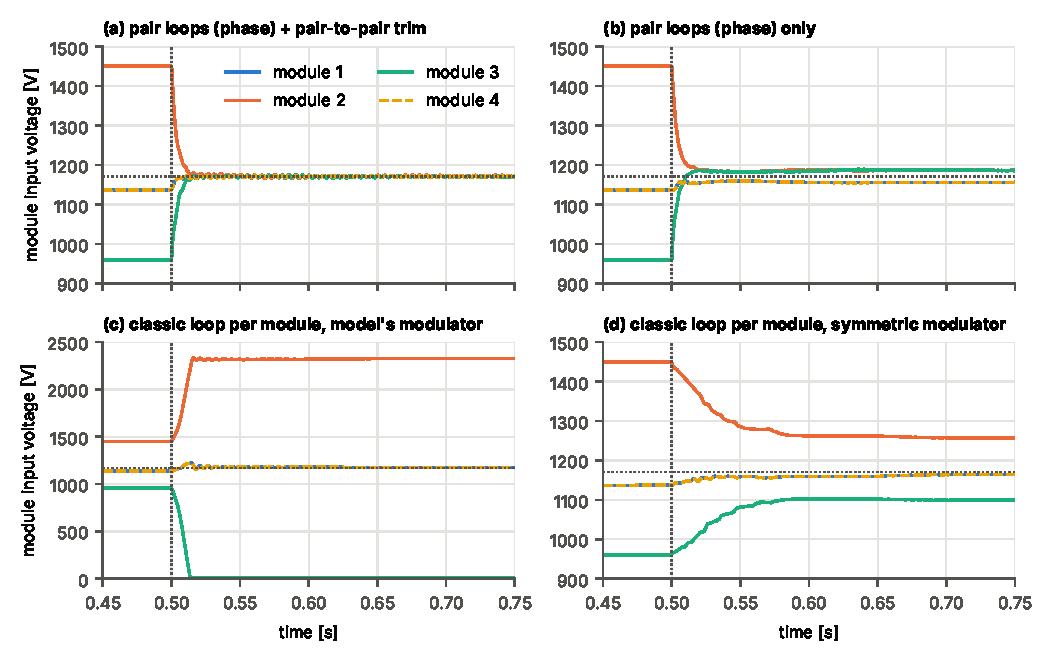
\includegraphics[width=0.94\textwidth]{figures/fig_balancing.pdf}
\caption{Module input voltages with \SI{20}{\percent} more leakage in module 2; the balancing loops start at \SI{0.5}{s} (switched simulation). (a) Pair loops on the relative phase and pair-to-pair trim of the phase shift. (b) Pair loops only. (c) Classic per-module loop on the phase shift with the modulator of the model (leg B moved): it diverges. (d) The same loop with a symmetric modulator: right direction, too weak.}
\label{fig:balancing}
\end{figure}

\begin{table}[!htb]
\centering
\caption{Balancing controls in the switched simulation: module input voltages \SI{0.5}{s} after the loops start, largest deviation from the mean, relative phase of the pair and phase-shift trim, time to come within \SI{2}{\percent}.}
\label{tab:balancing}
\small
\begin{tabular}{@{}llllll@{}}
\toprule
Case & Control & $v_1$, $v_2$, $v_3$, $v_4$ [V] & Deviation & $\varphi$, $d$ & Within \SI{2}{\percent} \\
\midrule
$L_{s2}$ \SI{+20}{\percent} & none & 1137, 1450, 959, 1137 & \SI{23.9}{\percent} & -- & -- \\
 & pair loops + trim & 1171, 1171, 1171, 1171 & \SI{0.07}{\percent} & \ang{2.5}, $\pm 0.007$ & \SI{10}{ms} \\
 & pair loops only & 1157, 1186, 1185, 1157 & \SI{1.2}{\percent} & \ang{2.5}, -- & \SI{16}{ms} \\
 & classic, model modulator & 1173, 2328, 8, 1173 & \SI{99}{\percent} & --, at the limit & diverges \\
 & classic, symmetric modulator & 1170, 1256, 1088, 1170 & \SI{7.3}{\percent} & --, at the limit & never \\
$L_{s2}$ \SI{+5}{\percent} & pair loops + trim & 1172, 1172, 1171, 1172 & \SI{0.16}{\percent} & \ang{0.7}, $\pm 0.004$ & \SI{5}{ms} \\
$n_1$ \SI{+2}{\percent} & pair loops + trim & 1170, 1170, 1170, 1171 & \SI{0.17}{\percent} & \ang{0}, $\pm 0.003$ & (\SI{1.5}{\percent} before) \\
equal modules & pair loops + trim & 1171 on each module & 0 & 0, 0 & -- \\
\bottomrule
\end{tabular}
\end{table}

The loops start at \SI{0.5}{s}, from the unbalanced steady state of Sect.~\ref{sec:sharing} (Fig.~\ref{fig:balancing}, Table~\ref{tab:balancing}). With \SI{20}{\percent} more leakage in module 2 the four input voltages come within \SI{2}{\percent} in \SI{10}{ms} and end within \SI{0.07}{\percent}, with $\varphi_{23} = \ang{2.5}$, against \ang{3.0} from \eqref{eq:kphi}, and $d = \pm 0.007$. The primary currents fall from \SI{606}{A} rms and \SI{900}{A} peak in module 2 to \SIrange{369}{389}{A} rms and at most \SI{514}{A} peak. The pair loops alone balance each pair but leave \SI{1.2}{\percent} between the pairs. With identical modules the loops do nothing.

\subsection{Practical notes}

\begin{itemize}
\item \textbf{Average the measured voltages over a switching period.} The control samples twice per period. A trim that differs between the two half periods gives unequal volt-seconds and a DC magnetizing current; the DC current makes the two half periods of the input current different, and the next samples see that difference. Without the average, the case with \SI{2}{\percent} more turns in module 1 builds up \SI{-115}{A} of DC magnetizing current in modules 1 and 4 in \SI{0.5}{s}, still growing; with the average it stays at the few amperes left from the start. The phase offsets move both legs together and do not change the volt-seconds; the trim of the phase shift does.
\item \textbf{Modulator.} One carrier per bridge with a phase input, and a phase-shift input per pair. The offsets are small (\ang{2.5} is \SI{1.7}{\micro s} at \SI{4}{kHz}), so the PWM needs a fine time resolution. A DSP timer has it; the simulation with its \SI{0.625}{\micro s} step still works because the loop dithers between two steps.
\item \textbf{Turns mismatch.} The pair loop makes the input voltages equal, not the secondary voltages: with \SI{2}{\percent} more turns in module 1 a reactive current circulates in the pair (module 1: \SI{393}{A} rms and \SI{501}{A} peak instead of \SI{381}{A} and \SI{463}{A}). Within normal tolerances this is small.
\item With one rectifier per module no pair loop is needed: the classic per-module loop, or no loop at all, is enough.
\end{itemize}

% =====================================================================================================
\section{Start, flux balance and voltage loop}
\label{sec:start}

\begin{figure}[!htb]
\centering
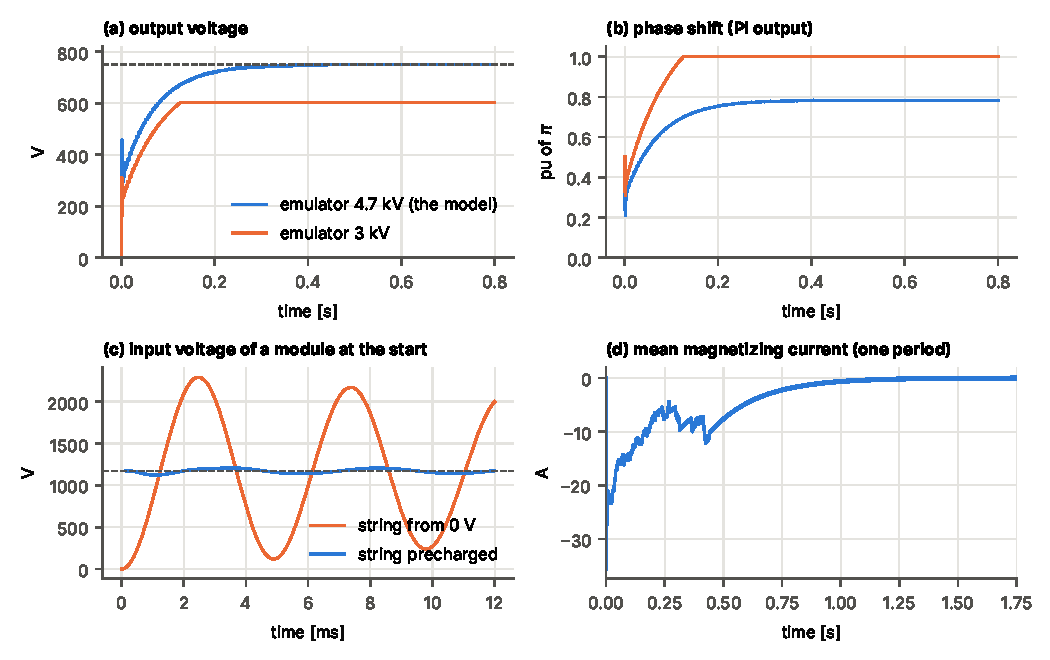
\includegraphics[width=0.86\textwidth]{figures/fig_start.pdf}
\caption{Start (switched simulation). (a) Output voltage and (b) phase shift with the emulator of the model and with the emulator at \SI{3}{kV}. (c) Input voltage of a module with the string precharged and from \SI{0}{V}. (d) Mean magnetizing current of a transformer.}
\label{fig:start}
\end{figure}

\textbf{Start.} The model starts from the DC steady state of the network (string precharged); the output reaches \SI{95}{\percent} of \SI{750}{V} in \SI{178}{ms} without overshoot (Fig.~\ref{fig:start}a,b), and the input filter (\SI{2}{mH} with the four capacitors in series, \SI{205}{Hz}) rings a little at the start. If the string capacitors start at \SI{0}{V} (their initial target in the model), the input filter rings up to \SI{2290}{V} per module, twice the nominal, with \SI{1.8}{kA} in the string (Fig.~\ref{fig:start}c): the real system needs a precharge of the string and a soft start of the reference.

\textbf{DC magnetizing current.} The phase shift changes at every half period during the start; each change between a positive and a negative half period gives unequal volt-seconds on the transformer and a step of DC magnetizing current. They add up to \SI{-21}{A}, \SI{40}{\percent} of the \SI{52}{A} AC peak, which decays only through the winding and switch resistances ($L_m/R \approx \SI{0.2}{s}$, Fig.~\ref{fig:start}d); with a real core this is a saturation risk. The "DC transformer current" PI of the model cannot correct it: its output is not connected, it measures the input current of the string (a DC current by nature) and it acts on the duty of both legs together, which gives no DC voltage on the transformer. A flux balance needs the DC part of each primary current and a differential action on the two legs; the usual alternatives are a DC-blocking capacitor in series with each primary or peak-current-mode control.

\textbf{Voltage loop.} With the averaged plant (gain $n\,v_k/\SI{750}{V}$ reduced by the droop of $\Req$: \num{1.29} pu/pu), the output filter and 1.5 samples of delay, the gains of the model give a crossover of \SI{4.8}{Hz} (phase margin \ang{129}, gain margin \SI{9.1}{dB}, closed-loop pole \SI{-14}{rad/s}). The proportional gain is limited by the resonance of the output filter at \SI{411}{Hz}: with $k_p = 0.8$ the loop crosses over at the resonance (\SI{511}{Hz}, gain margin \SI{4.9}{dB}). A faster loop needs more integral gain: $k_p = 0.6$, $k_i = \SI{100}{s^{-1}}$ gives \SI{33}{Hz}, \ang{135}, \SI{7.2}{dB} and a pole five times faster. Faster still, the input filter (characteristic impedance \SI{2.6}{\ohm}) must be checked against the \SI{-19.5}{\ohm} constant-power input of the converter \cite{middlebrook1976}.


% =====================================================================================================
\section{Summary}
\label{sec:summary}

\begin{itemize}
\item A phase-shift module behaves on average like $n D v_k$ behind the lossless resistance $\Req = 4n^2\Ls f$; with a common phase shift this resistance balances the input voltages of ISOP modules on separate rectifiers in about a millisecond.
\item Two modules whose transformers are paralleled on the AC side are tied through leakage reactances, so a voltage difference gives only reactive current: in \code{ps\_isop\_rail} the sharing inside a pair is about 23 times slower and a \SI{5}{\percent} leakage difference splits the voltages by \SI{\pm 15}{\percent}. One rectifier per module or a pair loop on the relative phase fixes it; a common-core four-winding transformer does not.
\item A loop per pair on the relative phase of its two bridges (a few degrees, \SI{40}{Hz} crossover) plus a slow trim of the phase shift between the pairs keeps the four input voltages within \SI{0.2}{\percent}, even with \SI{20}{\percent} more leakage in one module. The classic per-module loop on the phase shift has the wrong sign inside a pair with the modulator of the model. The measured voltages must be averaged over a switching period, or the trims build up a DC magnetizing current.
\item With $n = 1$ and a DAB-style leakage the output reaches \SI{750}{V} only with the emulator at $1.5$ times the catenary; a PSFB needs the turns ratio from the lowest catenary voltage and a small leakage.
\item The start needs a precharge; the DC magnetizing current left by the start is not controlled; the voltage loop is slow and its proportional gain is limited by the output filter.
\end{itemize}

{\small
\begin{thebibliography}{9}
\bibitem{en50163} EN~50163, \emph{Railway applications --- Supply voltages of traction systems}, CENELEC.
\bibitem{sabate1990} J.~A.~Sabaté, V.~Vlatkovic, R.~B.~Ridley, F.~C.~Lee, B.~H.~Cho, ``Design considerations for high-voltage high-power full-bridge zero-voltage-switched PWM converter,'' in \emph{Proc. IEEE APEC}, 1990, pp.~275--284.
\bibitem{giri2006} R.~Giri, R.~Choudhary, R.~Ayyanar, N.~Mohan, ``Common-duty-ratio control of input-series connected modular DC--DC converters with active input voltage and load-current sharing,'' \emph{IEEE Trans. Ind. Appl.}, vol.~42, no.~4, pp.~1101--1111, 2006.
\bibitem{ayyanar2004} R.~Ayyanar, R.~Giri, N.~Mohan, ``Active input-voltage and load-current sharing in input-series and output-parallel connected modular DC--DC converters using dynamic input-voltage reference scheme,'' \emph{IEEE Trans. Power Electron.}, vol.~19, no.~6, pp.~1462--1473, 2004.
\bibitem{dedoncker1991} R.~W.~De~Doncker, D.~M.~Divan, M.~H.~Kheraluwala, ``A three-phase soft-switched high-power-density DC/DC converter for high-power applications,'' \emph{IEEE Trans. Ind. Appl.}, vol.~27, no.~1, pp.~63--73, 1991.
\bibitem{middlebrook1976} R.~D.~Middlebrook, ``Input filter considerations in design and application of switching regulators,'' in \emph{Proc. IEEE IAS Annual Meeting}, 1976, pp.~366--382.
\end{thebibliography}
}

\end{onehalfspace}
\end{document}
